\title{Lecture 15\\Structuring Knowledge Bases Using a Hierarchy of Ontologies}

\begin{frame}
	\titlepage
\end{frame}

\begin{frame}{\\Lecture outline}
	\topline
	\justifying
	Knowledge base sections, their types, and their hierarchy. Atomic and non-atomic sections, section decomposition, and child sections. Top-level subject domains and ontologies and how they relate to each other.
\end{frame}

\begin{frame}{\\Structuring a knowledge base}
	\topline
	\justifying
	\begin{SCn}
		\textbf{Aspects of knowledge base structuring}
		\begin{textitemize}
			\item Hierarchy of subject domains and ontologies.
			\item Didactic (logical) structuring.
			\item Structuring to support the development process.
		\end{textitemize}
		\scnheader{didactic structuring}
		\scnidtf{structuring that takes into account how end users understand the knowledge}
		\scntext{note}{Didactic structuring must preserve the meaning of the knowledge.}
	\end{SCn}
\end{frame}

\begin{frame}{\\The concept of a knowledge base section}
	\topline
	\justifying
	The knowledge base of each OSTIS system is divided into sections. The concept of a section is a sign that denotes the set of all possible sections across knowledge bases.
	\bigskip

	Each section is a fragment of a knowledge base identified for \textit{didactic} purposes. It is \textit{logically coherent and self-contained}.

	The entire knowledge base of an OSTIS system can also be treated as a single non-atomic section.
\end{frame}

\iffalse
\begin{frame}{\\Relations on the set of sections}
	\topline
	\justifying
	\begin{SCn}
		\scnheader{relations on the set of sections}
		\scnhaselement{section decomposition*}
		\begin{scnindent}
			\scnidtf{quasi-binary directed relation between a section and the set of its subsections}
			\scnidtf{relation that defines the didactic structure of a section}
			\scntext{note}{The basic decomposition* relation links an \textbf{entity} to other \textbf{entities} that are its parts. The section decomposition* relation restricts this to a \textbf{section} and its \textbf{subsections}.}
		\end{scnindent}
		\scnhaselement{basic order of sections*}
		\begin{scnindent}
			\scnidtf{binary relation between sections that determines their order within a section decomposition}
		\end{scnindent}
	\end{SCn}
\end{frame}
\fi

\begin{frame}{\\Types of knowledge base sections}
	\topline
	\justifying
	\begin{SCn}
		\scnheader{section}
		\scnidtf{knowledge base section}
		\begin{scnrelfromset}{partition}
			\scnitem{non-atomic section}
			\scnitem{atomic section}
		\end{scnrelfromset}
		\scnsuperset{rationale section}
		\scnsuperset{principles section}
		\scnsuperset{documentation section}
		\scnsuperset{subject domain description section}
		\scnsuperset{semantic neighborhood description section}
	\end{SCn}
\end{frame}

\begin{frame}{\\Rationale, principles, and documentation}
	\topline
	\justifying
	\begin{SCn}
		\scnheader{rationale section}
		\scnidtf{formal text that explains why something should be developed by stating the problem, identifying shortcomings in existing solutions, describing the advantages of proposed solutions, and so on}

		\scnheader{principles section}
		\scnidtf{description of the fundamental principles behind the design or operation of a technology, subsystem, or similar entity}

		\scnheader{documentation section}
		\scnidtf{description of the purpose, usage principles, structure, and components of a system or subsystem}
	\end{SCn}
\end{frame}

\begin{frame}{\\Domain and neighborhood descriptions}
	\topline
	\justifying
	\begin{SCn}
		\scnheader{subject domain description section}
		\scnidtf{section containing the sign of the subject domain, the signs of all its elements, and its full specification, including all its ontologies}

		\scnheader{semantic neighborhood description section}
		\scnidtf{section containing the sign of a structure that is the semantic neighborhood of an sc-element, the signs of all its elements, and the specification of that structure}
	\end{SCn}
\end{frame}

\begin{frame}{\\Atomic and non-atomic sections}
	\topline
	\justifying

	The concept of a non-atomic section denotes the set of all non-atomic sections in various bodies of documentation. These are sections that can be decomposed into smaller sections. The entire knowledge base of an OSTIS system can also be treated as a single non-atomic section.
	\bigskip

	The concept of an atomic section denotes the set of all atomic sections in various bodies of documentation. These sections cannot be decomposed into smaller sections. Any concept that appears in an atomic section but does not play a key role there must play a key role in some other atomic section of the same knowledge base.
\end{frame}

\begin{frame}{\\Hierarchy of sections}
	\topline
	\justifying
	\begin{SCn}
		\scnheader{knowledge base section}
		\scntext{note}{The section hierarchy is defined by the relations \textit{child subject domain*}, \textit{child subject domain and ontology*}, and \textit{child section*}.}

		\scnheader{Section: Subject domain of knowledge and knowledge bases}
		\scnrelfrom{child section}{Section: Subject domain of sets}
	\end{SCn}
\end{frame}

\begin{frame}{\\Knowledge base fragment}
	\topline
	\justifying
	\begin{SCn}
		\scnheader{designated knowledge base fragment}
		\begin{scnrelfromset}{partition}
			\scnitem{family of knowledge base sections}
			\scnitem{knowledge base section}
			\scnitem{knowledge base segment}
			\scnitem{knowledge base fragment}
		\end{scnrelfromset}

		\scnheader{knowledge base section}
		\begin{scnrelfromset}{partition}
			\scnitem{atomic knowledge base section}
			\scnitem{non-atomic knowledge base section}
			\begin{scnindent}
				\scnidtf{section that is divided into segments}
			\end{scnindent}
		\end{scnrelfromset}
	\end{SCn}
\end{frame}

\begin{frame}{\\Sections, segments, and fragments}
	\topline
	\justifying
	\begin{SCn}
		\scnheader{knowledge base section}
		\scnsuperset{subject domain and ontology}
		\scnsuperset{subject domain fragment}
		\scnsuperset{specialized ontology}
		\scnsuperset{integrated ontology}
		\scnsuperset{subject domain}

		\scnheader{knowledge base segment}
		\scnidtf{part of a non-atomic knowledge base section}
		\scntext{note}{Knowledge base segments cannot have a hierarchical structure. In particular, they cannot consist of lower-level segments.}

		\scnheader{knowledge base fragment}
		\scnidtf{part of a knowledge base section}
	\end{SCn}
\end{frame}

\begin{frame}{\\Segments and fragments of a section}
	\topline
	\justifying
	\begin{SCn}
		\vspace{3em}
		\begin{figure}[H]
			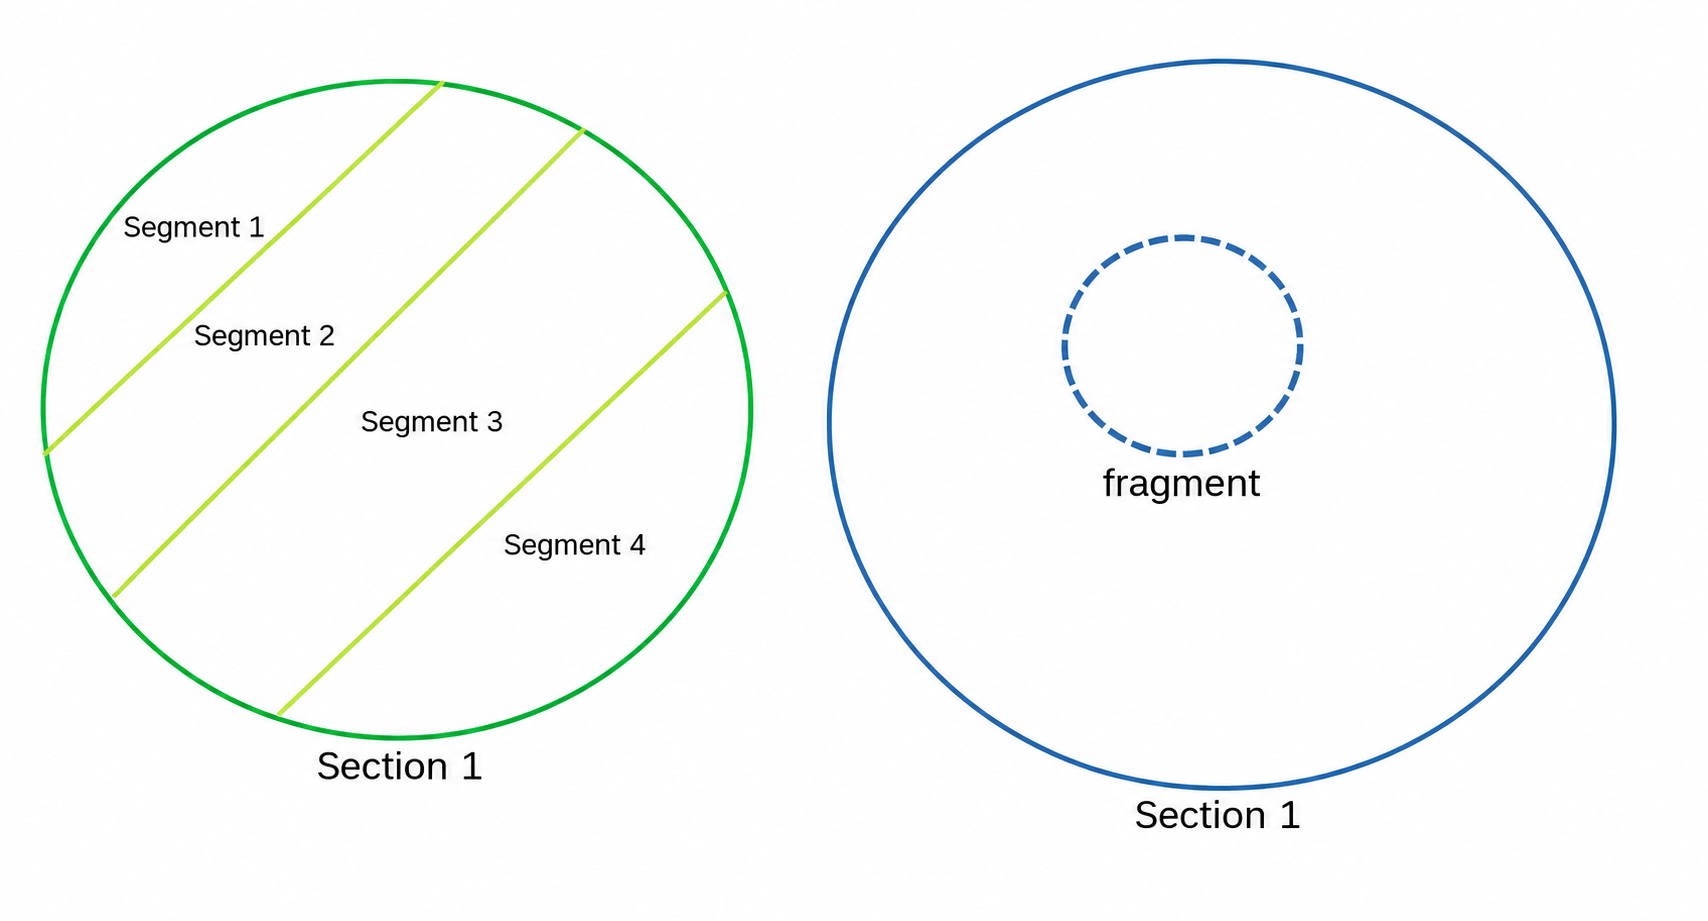
\includegraphics[width=0.74\linewidth,height=0.40\textheight,keepaspectratio]{figures/sd_structuring/segment_en.png}
		\end{figure}
		\vspace{-0.8em}
		\begin{columns}[T,onlytextwidth]
			\begin{column}{0.4\textwidth}
				\scnheader{Section 1}
				\begin{scnreltoset}{union}
					\scnitem{Segment 1}
					\scnitem{Segment 2}
					\scnitem{Segment 3}
					\scnitem{Segment 4}
				\end{scnreltoset}
			\end{column}
			\begin{column}{0.4\textwidth}
				\scnheader{Section 1}
				\scnsuperset{Fragment 1}
			\end{column}
		\end{columns}
	\end{SCn}
\end{frame}

\begin{frame}{\\Designated knowledge base fragment}
	\topline
	\justifying
	\begin{SCn}
		\scnheader{designated knowledge base fragment}
		\begin{scnrelfromset}{partition}
			\scnitem{named knowledge base fragment}
			\begin{scnindent}
				\scnsuperset{knowledge base section}
				\scnsuperset{knowledge base segment}
			\end{scnindent}
			\scnitem{unnamed knowledge base fragment}
		\end{scnrelfromset}

		\scnheader{family of knowledge base sections}
		\scnidtf{set of knowledge base sections}

		\scnheader{non-atomic knowledge base section}
		\scnidtf{section that is not itself a set of knowledge base segments}
	\end{SCn}
\end{frame}

\begin{frame}{\\Example}
	\topline
	\justifying
	\begin{SCn}
		\scnheader{Polygons}
		\scniselement{family of sections}
		\begin{scneqtoset}
			\scnitem{Triangles\\
			\begin{scnindent}
				\scniselement{non-atomic knowledge base section}
				\begin{scnreltoset}{concatenation of segments}
					\scnitem{Classification of triangles}
					\scnitem{Relations on triangles}
					\scnitem{Properties of triangles}
				\end{scnreltoset}
			\end{scnindent}}
			\scnitem{Quadrilaterals\\
			\begin{scnindent}
				\scniselement{atomic section}
			\end{scnindent}}
			\scnitem{Regular polygons\\
			\begin{scnindent}
				\scniselement{atomic section}
			\end{scnindent}}
		\end{scneqtoset}
	\end{SCn}
\end{frame}

\begin{frame}{\\Relations on designated fragments}
	\topline
	\justifying
	\begin{SCn}
		\scnheader{relations on the set of designated fragments}
		\scnhaselement{concatenation of segments*}
		\scnhaselement{child knowledge base fragment*}
		\begin{scnindent}
			\scnsuperset{child fragment of a knowledge base section*}
			\scnsuperset{child knowledge base section*}
			\begin{scnindent}
				\scntext{note}{The relation \textit{child knowledge base section*} is distinct from \textit{inclusion*} and \textit{child subject domain*}.}
			\end{scnindent}
		\end{scnindent}
	\end{SCn}
\end{frame}

\begin{frame}{\\Relations on designated fragments}
	\topline
	\justifying
	\begin{SCn}
		\scnheader{relations on the set of designated fragments}
		\scnhaselement{abstract*}
		\scnhaselement{preface*}
		\scnhaselement{introduction*}
		\scnhaselement{conclusion*}
		\scnhaselement{findings*}
		\scnhaselement{epigraph*}

		\scnheader{didactic relations}
		\scnhaselement{explanation*}
		\scnhaselement{note*}
		\scnhaselement{similarities*}
		\scnhaselement{comparison*}
		\scnhaselement{difference*}
		\scnhaselement{should be distinguished from*}
	\end{SCn}
\end{frame}

\begin{frame}{\\Didactic relations}
	\topline
	\justifying
	\begin{SCn}
		\scnheader{didactic relations}
		\scntext{explanation}{These relations are redundant in the knowledge representation itself, but they help present the knowledge in a way that is easier for users to understand.}
	\end{SCn}
\end{frame}

\begin{frame}{\\Top-level subject domains}
	\topline
	\justifying

	In top-level subject domains, the classes of objects of study are the broadest classes of entities, also called categories. Examples include:
	\begin{textitemize}
		\item the class of all parameters
		\item the class of all structures
		\item the class of all connections
		\item the class of all sets
		\item the class of all kinds of knowledge
	\end{textitemize}

	A subject domain can be associated with ontologies of different kinds that describe its concepts and clarify their meaning.
\end{frame}

\begin{frame}{\\Top-level ontologies}
	\topline
	\justifying

	An ontology associated with a top-level subject domain is called a top-level ontology. It organizes knowledge about the real world independently of any particular subject domain.
	\bigskip

	The main purpose of top-level ontologies is to support semantic compatibility between subject domain ontologies and application ontologies. They provide a common basis for formulating definitions. Terms in domain-specific ontologies are subordinate to terms in a higher-level ontology.
\end{frame}
